\chapter{Dischi in sistemi binari}
Il collasso dei cores nelle nubi molecolari porta nel $50\%$ dei casi \parencite{FreqMultipli} alla formazione di sistemi multipli, ossia composti da più stelle che orbitano attorno al centro di massa totale.
Questi studi sono rilevanti perché in questo lavoro di tesi ci focalizzeremo sui sistemi binari, che sono formati da due stelle che interagiscono gravitazionalmente fra loro. 

Per studiare l'evoluzione di una binaria è necessario il concetto di \textit{Roche lobe}, che è la regione di spazio all'interno della quale il materiale orbitante è gravitazionalmente legato alla stella selezionata.
Il raggio di Roche-Lobe $R_L$ dipende solamente dal mass-ratio $q\,=\,m_2/m_1$ e dal semiasse maggiore dell'orbita $a$ \parencite{Eggleton1983}:
\begin{equation}
R_L\,=\,a \cdot \frac{0.49 \cdot q^{-2/3}}{0.6 \cdot q^{-2/3}\,+\,\ln{(1\,+\,q^{-1/3})}}.
\label{eq:roche_lobe_ras}
\end{equation}
Sono allora possibili tre configurazioni per un sistema binario:
\begin{list}{\textbf{-}}{\setlength{\itemsep}{0cm}}
    \item 'detached binary', in cui nessuna delle due stelle riempie il proprio Roche-Lobe
    \item 'semi-detached binary', in cui una delle due stelle riempie il proprio Roche-Lobe
    \item 'contact binary', in cui entrambe le stelle riempiono il loro Roche-Lobe. In questo caso il sistema stellare appare come un singolo oggetto caratterizzato dalla presenza di due cores stellari legati insieme da uno strato comune.
\end{list}
In Figura \ref{fig:roche_lobe} è riportato il caso di un sistema in cui nessuno dei due Roche-Lobe è pienamente occupato.
\begin{figure}[h]
  \centering
  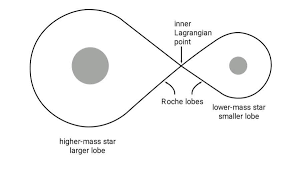
\includegraphics[width=0.7\textwidth]{Immagini/IntroTeorica/RocheLobe.png}
  \caption{In questo esempio entrambe le stelle si trovano all'interno del loro Roche-Lobe (tracciato in nero). Notiamo che le due regioni delimitate dalla linea continua si incontrano nel punto di Lagrange posizionato lungo la congiungente fra i due corpi. Tale posizione è quella in cui le attrazioni gravitazionali da parte delle due stelle si elidono a vicenda. }
  \label{fig:roche_lobe}
\end{figure}

Un sistema binario può presentare tre dischi proto-planetari separati: due circum-stellari (ognuno attorno ad una stella) ed uno circum-binario, che orbita attorno al centro di massa della binaria. La casistica dei dischi è rilevante solo per le binarie che non riempiono il proprio \textit{Roche-Lobe}.
\begin{figure}[h]
    \centering
    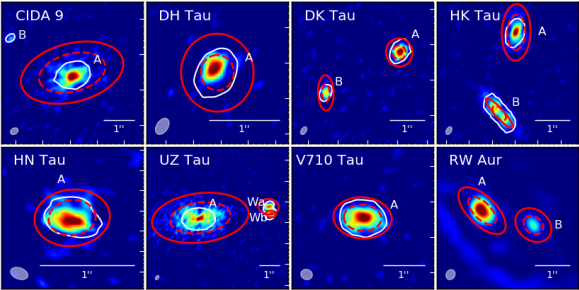
\includegraphics[height=6cm, width=14cm]{Immagini/IntroTeorica/DischiRota.png}
    \caption{Immagini delle emissioni di $^{12}$CO di dischi attorno a sistemi multipli nella nebulosa del Toro. Sono riportati gli ellissi che racchiudono il 68 \% (linea tratteggiata) ed il 95 \% del flusso totale (linea continua). In ogni figura è presente una barra, di lunghezza 1'' \parencite{OsservazioniRota}.}
    \label{fig:oss_rota}
\end{figure}
In un tale sistema le parti esterne dei dischi circum-stellari sono influenzate da effetti mareali dovuti alla presenza dell'altro corpo: tali interazioni solitamente portano al troncamento del disco.
Questo fenomeno è causato dal fatto che in sistemi a più corpi le interazioni dinamiche fra materiale gassoso e stelle determinano lo svuotamento di certe regioni spaziali.
Dal punto di vista osservativo i dischi in sistemi multipli sono fonte di emissioni più deboli (nel sub-millimetrico) rispetto a quelli nei sistemi singoli \parencite{DimDisc}.
Il disco circum-primario è solitamente più massivo e più luminoso del disco circum-secondario. In Figura \ref{fig:oss_rota} sono riportate delle osservazioni di dischi circumstellari in sistemi binari appartenenti alla nebulosa del Toro.


\section{Cenni sul problema di Keplero} \label{sec:Keplero}

Il problema fisico che andiamo ad affrontare è quello di due punti materiali di massa $m_1$ ed $m_2$ rispettivamente posti in $\Vec{x}_1$ ed $\Vec{x}_2$, che interagiscono tra loro con una forza diretta lungo la congiungente e dipendente solo dalla loro distanza.
La lagrangiana del sistema usando coordinate cartesiane è:
\begin{equation}
L\left(\textbf{x}_1,\,\textbf{x}_2,\,\dot{\textbf{x}}_1,\,\dot{\textbf{x}}_2\right)\,=\,\frac{1}{2}m_1\left|\dot{\textbf{x}}_1\right|^2\,+\,\frac{1}{2}m_2\left|\dot{\textbf{x}}_2\right|^2\,-\,V\left(\left|\textbf{x}_1\,-\,\textbf{x}_2\right|\right).
\label{eq:lag_cartesiane}
\end{equation}
Notiamo che la \eqref{eq:lag_cartesiane} è invariante per traslazioni rigide poiché il potenziale dipende solamente da $\left|\textbf{x}_1\,-\,\textbf{x}_2\right|$: conviene utilizzare un sistema di riferimento che renda più evidente questa simmetria. Definiamo allora la coordinata relativa $\textbf{x}_{rel}$, dalla quale dipenderà il potenziale $V$ e la coordinata del centro di massa $\textbf{x}_{CM}$:
\begin{equation}
\textbf{x}_{rel}\,=\,\textbf{x}_1\,-\,\textbf{x}_2,
\label{eq:x_rel}
\end{equation}
\begin{equation}
\textbf{x}_{CM}\,=\,\frac{m_1\textbf{x}_1\,+\,m_2\textbf{x}_2}{m_1\,+\,m_2}.
\label{eq:x_centermass}
\end{equation}
Applicando il precedente cambio di coordinate è possibile scrivere la lagrangiana di partenza come somma di una parte baricentrale ed una relativa
\begin{equation}
L\left(\dot{\textbf{x}}_{CM},\,\textbf{x}_{rel},\,\dot{\textbf{x}}_{rel}\right)\,=\,\frac{1}{2}M\left|\dot{\textbf{x}}_{CM}\right|^2\,+\,\frac{1}{2}\mu\left|\dot{\textbf{x}}_{rel}\right|^2\,-\,V\left(\textbf{x}_{rel}\right),
\label{eq:lag_cambiocoor}
\end{equation}
dove $M\,=\,m_1\,+\,m_2$ e $\mu$ è la massa ridotta. Notiamo che non è presente alcuna dipendenza su $\textbf{x}_{CM}$: per il teorema di Nother i momenti associati a tale coordinata sono conservati. Le informazioni importanti riguardo l'evoluzione del sistema sono da ricercare nella lagrangiana relativa:
\begin{equation}
L_{rel}\left(\textbf{x}_{rel},\,\dot{\textbf{x}}_{rel}\right)\,=\,\frac{1}{2}\mu\left|\dot{\textbf{x}}_{rel}\right|^2\,-\,V\left(\textbf{x}_{rel}\right).
\label{eq:lag_rel}
\end{equation}
La \eqref{eq:lag_rel} può essere ridotta ad un sistema ad un solo grado di libertà lavorando in un sistema di riferimento polare. Consideriamo il cambio di coordinate:
\begin{equation}
\begin{cases}
x_{rid}\,=\,r\cos{\varphi} \sin{\theta} \\
y_{rid}\,=\,r\sin{\varphi} \sin{\theta} \\
z_{rid}\,=\,r\cos{\theta}
\end{cases}
\label{eq:cambiocoor_rel}
\end{equation}
ottenendo per la lagrangiana ridotta l'espressione
\begin{equation}
\Tilde{L}_{rid}(r,\,\theta,\,\dot{r},\,\dot{\varphi},\,\dot{\theta})\,=\,\frac{1}{2}\mu(\dot{r}^2\,+\,r^2 \sin^2\theta\dot{\varphi}^2\,+\,r^2\dot{\theta}^2)\,-\,V\left(r\right).
\label{eq:lag_rel_pol}
\end{equation}
Il potenziale $V(r)$ è centrale e di conseguenza il momento angolare $\textbf{L}$ del sistema è conservato. Detto $J$ il momento angolare iniziale, è possibile mostrare che la \eqref{eq:lag_rel_pol} può essere scritta in dipendenza della sola coordinata radiale
\begin{equation}
\Tilde{L}_{rid}(r,\,\dot{r})\,=\,\frac{1}{2}\mu\dot{r}^2\,-\,V_J\left(r\right),
\label{eq:lag_solor}
\end{equation}
dove il $V_J(r)$ assume la forma
\begin{equation}
V_J(r)\,=\,\frac{J^2}{2\mu r^2}\,+\,V(r).
\label{eq:pot_eff_kepl}
\end{equation}
Un potenziale di questo genere può comportare orbite aperte oppure chiuse in dipendenza dei parametri che caratterizzano il moto dei corpi. In Figura \ref{fig:ritr_fase} è riportato il ritratto in fase per $J \neq 0$. Notiamo che possiamo avere tre tipi di orbite:
\begin{list}{\textbf{-}}{\setlength{\itemsep}{0cm}}
    \item circolari in corrispondenza del minimo
    \item limitate per valori di energia tali per cui $V_J(r_{min}) < E < 0$
    \item illimitate per $E \geq 0$
\end{list}
Le orbite limitate per il problema in questione sono o circonferenze o ellissi in cui il centro di massa del sistema occupa uno dei due fuochi. I parametri che consentono di descrivere le traiettorie sono l'eccentricità $e$ ed il semi-asse maggiore $a$: noti momento angolare $L$ ed energia $E$ del sistema è possibile ricavarli come
\begin{equation}
a\,=\,-\frac{Gm_1m_2}{2E_{tot}},
\label{eq:semiasse_mag}
\end{equation}
\begin{equation}
e\, = \sqrt{1\,-\,\frac{J^2}{GMa\mu^2}}.
\label{eq:ecc_kepl}
\end{equation}

\begin{figure}[H]
  \centering
  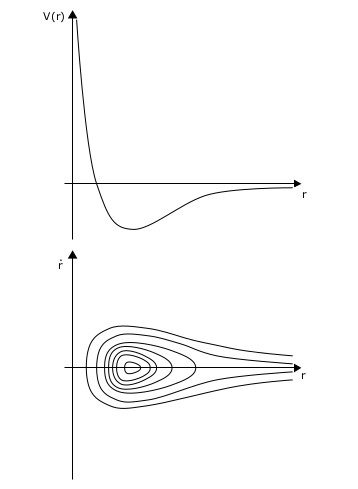
\includegraphics[width=0.7\textwidth]{Immagini/IntroTeorica/RitrattoFase.png}
  \caption{Ritratto in fase per il sistema studiato. Il potenziale efficace $V_{eff}(r)$ presenta un minimo globale che corrisponde ad un moto circolare uniforme. Per energie negative l'orbita è chiusa, ma con velocità radiale variabile nel tempo.}
  \label{fig:ritr_fase}
\end{figure}

\section{Fisica del troncamento} \label{sec:fis_tronc}

Le interazioni fra un disco gassoso ed un compagno perturbante possono essere studiate con approcci differenti:
\begin{list}{\textbf{-}}{\setlength{\itemsep}{0cm}}
    \item in termini di forze di marea \parencite{PapaloizouPringle1977}, lavorando con l'\textit{impulse approximation} \parencite{LinPapaloizou1979}
    \item assumendo che le interazioni vengano eccitate in particolari posizioni spaziali, dette risonanze
    \item considerando le orbite di particelle test e la loro stabilità
\end{list}

\subsection{Troncamento mareale}

Vogliamo valutare gli effetti delle perturbazioni mareali su un disco d'accrescimento orbitante attorno alla stella primaria (massa $m_1$), dovute alla presenza del secondo corpo di massa $m_2$.
Lavoriamo assumendo che il mass ratio del sistema considerato sia piccolo: l'interazione di natura mareale presa in considerazione è debole.
Quando $m_2/m_1 \ll 1$ la forza attrattiva della secondaria viene percepita dal gas orbitante attorno ad $m_1$ solo quando $m_2$ è vicina: le particelle che risentono della presenza del secondo corpo sono solamente quelle al bordo del disco.
La traiettoria di un elemento viene deviata sotto l'azione della forza di marea di un angolo tale che 
\begin{equation}
\cot^2{\left(\frac{\delta}{2}\right)}\,=\,\frac{v^4b^2}{G^2m_2^2},
\label{eq:picc_ang}
\end{equation}
dove $v$ è la velocità relativa fra stella e gas, mentre $b$ è il parametro d'impatto. Dato che le particelle stanno orbitando attorno ad $m_1$ con una frequenza angolare $\Omega$ ed il periodo d'orbita della binaria è dato da $2\pi/\omega$ possiamo esplicitare $v\,=\,(\Omega\,-\,\omega)R$, dove con $R$ si intende l'estensione spaziale del disco finora ignota.
Per la casistica in analisi è possibile ricavare il tasso di trasferimento di momento angolare specifico $\dot{h}$ \parencite{LinPapaloizou1979}, che risulta
\begin{equation}
\dot{h}\,=\,\frac{G^2m_2^2}{\pi R^2 b^2 (\Omega\,-\,\omega)^2}.
\label{eq:rate_moma}
\end{equation}
Lavorando con un espansione di Taylor per $\Omega$ è possibile valutare il tasso di trasporto del momento angolare sull'intero disco
\begin{equation}
\dot{H}\,=\,\frac{2G^2m_2^2R\Sigma}{R^2(d\Omega/dR)^2}\int_B^\infty \frac{db}{b^4}\,=\,\frac{2G^2m_2^2\Sigma}{3RB^3(d\Omega/dR)^2},
\label{eq:rate_moma_alldisc}
\end{equation}
dove $\Sigma$ è la densità superficiale e $B$ il minimo valore che viene assunto da $b$. Possiamo ora determinare il tempo caratteristico per i fenomeni di natura mareale
\begin{equation}
\tau_{mar}\,=\,\frac{27\pi}{8}\left(\frac{B}{R}\right)^3\frac{1}{\Omega q^2}\frac{9\pi}{8q\Omega}.
\label{eq:t_mareale}
\end{equation}
Il passaggio della secondaria causa un cambiamento nelle orbite percorse dal materiale costituente il disco: esse da circolari diventano eccentriche.
Dopo un incontro ravvicinato con la binaria la forza di marea diventa molto debole: se i fenomeni viscosi sono abbastanza intensi il momento angolare verrà ridistribuito all'interno del disco per giungere nuovamente allo stato a minima energia del sistema con conseguente ricircolarizzazione delle orbite.
Dato che $m_2 \ll m_1$ nella regione di spazio vicino alla primaria è possibile trascurare le interazioni di marea: l'evoluzione del disco è di natura viscosa ed il materiale accresce sulla stella primaria poiché il momento angolare $L_{disco}$ viene portato verso l'esterno. 
I tempi scala dei fenomeni viscosi dipendono linearmente dal numero di Reynolds:
\begin{equation}
\tau_{visc}\,=\,\frac{R}{\Omega}.
\label{eq:t_viscoso}
\end{equation}
Il trasporto viscoso di momento angolare all'interno del disco comporta l'allontanamento di una certa frazione della massa dalla protostella centrale: tale fenomeno prosegue fino a quando $L_{disco}$ viene portato al bordo esterno del disco.
All'outer edge può succedere che:
\begin{list}{\textbf{-}}{\setlength{\itemsep}{0cm}}
    \item $\tau_{mar}\,>\,\tau_{visc}$, ossia gli effetti di natura viscosa sono ancora dominanti. In questo caso il disco continuerebbe ad espandersi.
    \item $\tau_{mar}\,<\,\tau_{visc}$, ossia la forza di marea è più efficiente dei fenomeni viscosi. In questo caso l'espansione del disco si blocca e l'eccesso di momento angolare viene donato alla binaria per mezzo dell'interazione di marea. Il disco viene troncato.
\end{list}

Il raggio di troncamento viene quindi individuato imponendo che $\tau_{mar}\,=\,\tau_{visc}$. Osserviamo dalle relazioni \eqref{eq:t_mareale}, \eqref{eq:t_viscoso} che $\tau_{mar} \propto 1/R^3$ e $\tau_{visc} \propto R$: cambiare la viscosità $\nu$ non comporterà un grande cambiamento del raggio di troncamento.

\subsection{Troncamento risonante}

Un approccio differente e più accurato rispetto a quello dell' \textit{impulse approximation} consiste nel lavorare considerando le interazioni fra disco e corpo perturbante come eccitate in regioni specifiche dello spazio \parencite{GoldreichTremaine1980}.
La teoria del troncamento risonante presuppone che le perturbazioni al potenziale centrale della stella attorno a cui orbita il disco circumstellare siano piccole, ossia che il disco si trovi lontano dal corpo perturbante. 
Tale assunzione non è sempre verificata, poiché è possibile avere interazioni intense in \textit{close interacting binary systems}.
Il potenziale di un sistema binario determinato dalla presenza di due stelle a simmetria sferica rispettivamente poste in $\Vec{r}_1$ ed $\Vec{r}_2$ risulta pari a 
\begin{equation}
\phi(r,\,\theta,\,t)\,=\,-\sum_{j=1}^2 \mu_j \frac{GM}{|\mathbf{r}\,-\,\mathbf{r}_j|},
\label{eq:pot_per}
\end{equation}
dove $\mathbf{r}$ indica la regione in cui viene calcolato il potenziale, $\mathbf{r}_j$ è la posizione del j-esimo corpo, $\mu_1\,=\,1\,-\,\mu$ e $\mu_2\,=\,\mu$.
L'assunzione di piccole perturbazioni ci permette di lavorare con metodi perturbativi lineari espandendo il potenziale \eqref{eq:pot_per} in serie di Fourier \parencite{GoldreichTremaine1980} come
\begin{equation}
\phi(r,\,\theta,\,t)\,=\,\sum_{l=-\infty}^{\infty} \sum_{m=0}^{\infty}\phi_{l,m}(r)\exp{[i(m\theta\,-\,l\Omega_{B}t)]},
\label{eq:esp_tay}
\end{equation}
dove l è il numero caratteristico dei modi normali temporali, $m \geq 0$ è il numero azimutale, $\phi_{l,m}(r)$ è la componente potenziale ed $\Omega_B\,=\,(GM/a^3)^{1/2}$ è la velocità angolare media della binaria ($M$ è la massa totale del sistema, mentre $a$ denota il semiasse maggiore). Notiamo che le singole armoniche del potenziale binario ruotano uniformemente con velocità angolare di pattern $\Omega_P\,=\,(l/m)\Omega_B$.

Invertendo la \eqref{eq:esp_tay} è possibile determinare $\phi_{l,m}$ \parencite{ArtymowiczLubow1994} come
\begin{equation}
\phi_{m,l}\,=\,\frac{1}{2\pi^2}\int_0^{2\pi}d(\Omega_Bt) \int_0^{2\pi} d\theta \phi \cos{(m\theta\,-\,l\Omega_Bt)}.
\label{eq:singpot_shape}
\end{equation}
Ogni armonica $\phi_{m,l}$ può dare origine a tre risonanze:
\begin{list}{\textbf{-}}{\setlength{\itemsep}{0cm}}
    \item una risonanza corotazionale, che si verifica per quel raggio tale per cui $\Omega(r)\,=\,(l/m) \cdot \Omega_{B}$
    \item due risonanze di Lindblad LR (una interna ILR ed una esterna OLR) per quelle posizioni radiali tali per cui $m(\Omega(r)\,-\,\Omega_p)\,=\,\mp k$
\end{list}
Una risonanza è detta di Lindblad se la forzante su una particella che si muove su un orbita imperturbata agisce alla frequenza epiciclica. Dato che stiamo lavorando con un disco quasi-Kepleriano le risonanze si sviluppano ad
\begin{equation}
r_{CR}\,=\,(m/l)^{2/3}\mu_\ast^{1/3}a,
\label{eq:pos_corot}
\end{equation}
\begin{equation}
r_{LR}\,=\,[(1\pm m)]^{2/3} \mu_\ast^{1/3}a,
\label{eq:pos_lind}
\end{equation}
dove il segno $+$ corrisponde alla \textit{Outer Lindblad Resonace}, il $-$ alla ILR e $\mu_\ast$ corrisponde alla frazione della massa della binaria presente al centro del disco. Notiamo che alcune risonanze non sono presenti in alcun possibile disco: le ILR $(m,\,l)\,=\,(1,\,l)$ sono poste a $r\,=\,0$, mentre le OLR $(m,\,l)\,=\,(m,\,0)$ dovrebbero essere poste ad infinito. Può essere verificato che le risonanze appena presentate non siano importanti per la determinazione del bordo del disco.\\

Conviene ora definire il parametro $k\,=\,m\,-\,l$. Si può dimostrare che il momento torcente associato alle risonanze IRL/OLR dipende dal quadrato del potenziale perturbante. Dato che $\phi_{m,m-k} \sim e^{|k|}$ \parencite{GoldreichTremaine1980}, i momenti torcenti risonanti scalano con l'eccentricità del sistema binario come $T_{l,m} \sim e^{2 |k|}$: i valori maggiori si hanno per $k\,=\,m\,-\,l\,=\,0$. Notiamo che le risonanze 'eccentriche' con $|k|\,>\,0$ diventeranno progressivamente più intense all'aumentare di $e$. 
In Figura \ref{fig:pos_ris} vengono indicate le posizioni delle risonanze più importanti presenti nei dischi circumstellari: la scelta $l\,+\,m/10$ serve solamente per separare le coppie $(m,\,l)$ fra loro e non ha alcun significato fisico.

\begin{figure}[h]
  \centering
  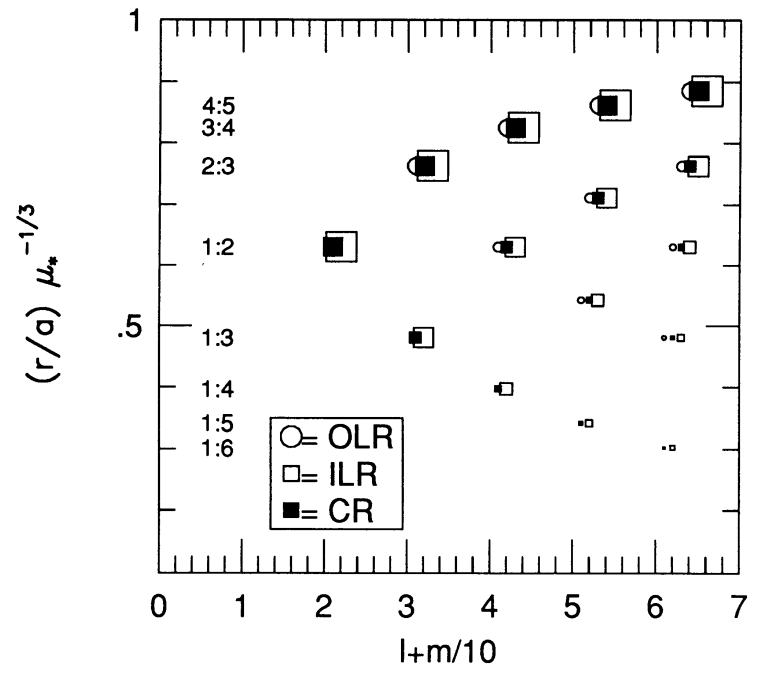
\includegraphics[width=0.7\textwidth]{Immagini/IntroTeorica/Risonanze_circumstellare.png}
  \caption{Posizioni delle LR e delle risonanze corotazionali in un disco circumstellare per diverse combinazioni $(m,\,l)$ tali da soddisfare la condizione $|k|\,=\,|m\,-\,l|\,<\,5$. Le risonanze più intense sono rappresentate dai simboli più grandi: la diminuzione delle loro dimensioni è dovuta alla diminuzione in intensità delle perturbazioni. Il disco circumstellare è posto attorno alla stella caratterizzata da $\mu_\ast$ \parencite{ArtymowiczLubow1994}. }
  \label{fig:pos_ris}
\end{figure}
Notiamo che sono presenti delle ILR molto intense oltre alla commensurabilità $1\,:\,2$: tali risonanze non sono importanti per le binarie con mass-ratio non estremi perché sono solitamente troppo intense e rimuovono sempre il materiale in corrispondenza della loro posizione spaziale.
Nei dischi circumstellari giocano un ruolo importante le risonanze caratterizzate da $m\,=\,2$, poiché sono le più interne.
\\

\textbf{Criteri per il gap-opening}\\

Il criterio per il \textit{gap opening} sviluppato da \textcite{ArtymowiczLubow1994} consiste nel valutare l'equilibrio fra i momenti torcenti di natura viscosa e quelli dovuti al corpo perturbante. Per far si che un disco venga troncato in una determinata posizione si deve avere che
\begin{equation}
3 \pi \alpha\left(\frac{h}{r}\right)^2\,\leq\,\frac{T}{\sigma \Omega^2 r^4},
\label{eq:crit_tronc}
\end{equation}
dove $T$ è il momento torcente esterno e $\sigma$ è la densità superficiale del disco nell'intorno del gap.
Il primo membro della condizione appena riportata è l'inverso del numero di Reynolds $R^{-1}$ del materiale orbitante moltiplicato per il fattore $3 \pi$, mentre il secondo membro è un momento torcente risonante specifico. Ricordiamo che in generale il gas costituente il disco ha $R\,\in\,\{10^{4},\,10^{6}\}$.
Oltre il verificarsi della condizione \eqref{eq:crit_tronc} è necessario che il tempo caratteristico per l'apertura del gap $t_{open}$ sia molto inferiore rispetto agli altri tempi caratteristici della binaria. Il criterio per il gap opening può essere riformulato \parencite{ArtymowiczLubow1994} come
\begin{equation}
\alpha^{1/2}\left(\frac{h}{r}\right)\,\leq\,\left(\frac{a|\phi_{lm}|}{GM}\right)\frac{(\pi m)^{1/2}(m\pm1)^{1/6}|\lambda\mp 2m|}{3\mu_\ast^{2/3}l^{2/3}},
\label{eq:crit_tronc1}
\end{equation}
dove $\lambda\,=\,[d\ln{\phi_{l,m}}/d\ln{r}]_{LR}$.\\

\textbf{Dimensioni dei dischi circumstellari}\\

Consideriamo la casistica di binaria circolare: vogliamo valutare quale rapporto fra le masse dei due corpi consenta di avere il disco troncato alla ILR caratterizzata da $(m,\,l)\,=\,(2,\,2)$. La componente $\phi_{2,2}(r)$ può essere espressa \parencite{ArtymowiczLubow1994} come
\begin{equation}
\phi_{22}(r)\,\simeq\,-\frac{3(1\,-\,\mu_\ast)GMe}{4a}\left(\frac{r}{a}\right)^2,
\label{eq:pot_22_bin}
\end{equation}
il che fornisce una condizione di bilanciamento dei momenti torcenti pari a
\begin{equation}
\alpha^{1/2}\left(\frac{h}{r}\right)\,=\frac{3\pi^{1/2}}{2^{5/2}}(1\,-\,\mu_\ast).
\label{eq:bil_22}
\end{equation}
Il numero di Reynolds caratteristico del materiale costituente un disco proto-planetario è $R \sim 10^{5}$ e l'aspect-ratio tipico è $h/r\,\sim\,0.1$ (vedi Sezione \ref{sec:mod_disc}): per far sì che l'uguaglianza \eqref{eq:bil_22} sia rispettata, è necessario che $1\,-\,\mu_\ast \lesssim 10^{-2}$.
Solitamente tali valori di $1\,-\,\mu$ sono verificati con pianeti giganti orbitanti attorno alla propria stella. I dischi in sistemi binari saranno di dimensioni nettamente inferiori. In Figura \ref{fig:dimdis_art} sono riportate le dimensioni dei dischi circumstellari per $\mu\,=\,0.3$ al variare del numero di Reynolds: l'estensione dei corpi rotanti sono determinate valutando il criterio del gap-opening per le risonanze $(m,\,l)\,=\,(2,\,l)$.
\begin{figure}[h]
    \centering
    
    \begin{subfigure}{0.48\textwidth}
        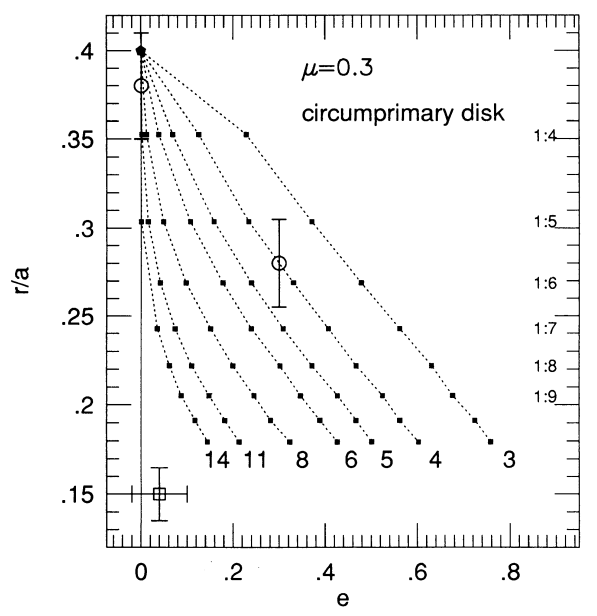
\includegraphics[width=\linewidth]{Immagini/IntroTeorica/DimPrim_Art_mu0.3.png}
    \end{subfigure}
    \hfill
    \begin{subfigure}{0.48\textwidth}
        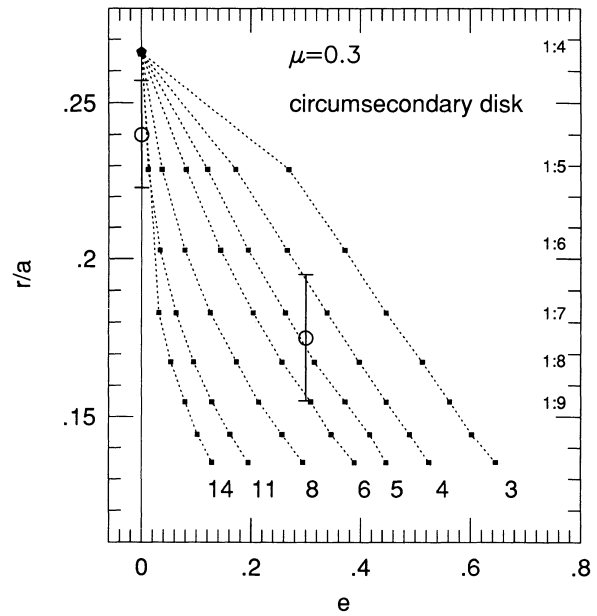
\includegraphics[width=\linewidth]{Immagini/IntroTeorica/DimSec_Art_mu0.3.png}
    \end{subfigure}
    
    \caption{In figura sono riportati i valori dei raggi dei dischi circumstellari per $\mu\,=\,0.3$, basati sulle posizioni delle varie risonanze. Le linee tratteggiate sono 7 e collegano i dati caratterizzati dallo stesso valore del numero di Reynolds: alla fine delle righe è riportato il valore di $\log{R}$. I cerchi con le barre d'errore sono i valori simulativi ottenuti da \textcite{ArtymowiczLubow1994}. Notiamo come al variare del numero di Reynolds, per avere il disco troncato nella stessa posizione è necessario che cambi l'eccentricità della binaria considerata \parencite{ArtymowiczLubow1994}.}
    \label{fig:dimdis_art}
\end{figure}

\subsection{Stable invariant loops}

Il metodo degli \textit{stable invariant loops} si focalizza sui cammini percorsi dalle particelle di gas: in un disco stabile tali traiettorie non devono intersecarsi fra loro o autointersecarsi. 
Il metodo sviluppato da \textcite{Pichardo2005} è focalizzato solamente su effetti di natura dinamica dell'interazione fra corpo perturbante ed anello di gas: tale approccio non consente di studiare gli effetti legati alla pressione ed alla viscosità del materiale orbitante.
Un \textit{stable invariant loop} consiste in un contorno chiuso nello spazio delle configurazioni tale per cui ogni punto inizialmente all'interno dello stesso evolve nel tempo ritornando nella condizione iniziale dopo un periodo della binaria.
Quando tali regioni di spazio non si intersecano fra loro possono essere riempite di gas: se il materiale guadagna o perde momento angolare  può attraversare diverse sequenze di invariant loops.

Un modo per identificare \textit{stable loops} consiste nell'effettare delle simulazioni numeriche \parencite{Pichardo2005}.
Procedendo in questo modo è possibile individuare diverse tipologie di traiettorie:
\begin{list}{\textbf{-}}{\setlength{\itemsep}{0cm}}
    \item orbite circumstellari
    \item orbite circumbinarie
    \item orbite che comportano l'allontanamento della particella dal sistema binario
    \item orbite che portano il materiale ad accrescere su una delle due stelle
\end{list}

Molto vicino alle stelle i \textit{stable loops} sono delle orbite circolari dovute alla presenza del corpo centrale: l'influenza della seconda componente della binaria può essere trascurata totalmente. Allontanandosi dal centro del sistema di riferimento considerato, le orbite tendono ad aumentare in eccentricità e a presentare una forma più allungata. In Figura \ref{fig:stable_loops_Pichardo} è riportato un esempio di calcolo dei stable loops.

\begin{figure}[h]
  \centering
  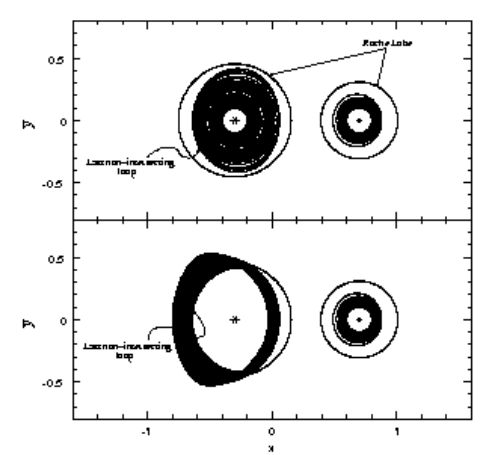
\includegraphics[width=0.7\textwidth]{Immagini/IntroTeorica/StableLoopsPichardo.png}
  \caption{Plot che riporta gli \textit{invariant loops} circumstellari per una binaria con: $q\,=\,0.2$, $e\,=\,0.0$. Nella parte superiore sono riportati tutti quei cicli fino all'ultimo non intersecante, mentre in quella inferiore sono riportati i \textit{loops} dal primo intersecante all'ultimo trovato. Notiamo come il passaggio da non intersecanti ad intersecanti avvenga intorno al raggio del Roche-lobe. \parencite{Pichardo2005}}
  \label{fig:stable_loops_Pichardo}
\end{figure}

I dischi circumbinari presentano un comportamento opposto: a grandi distanze dalla binaria, ossia per $r \gg a$ i \textit{stable loops} risultano essere circolari poiché con buona approssimazione è possibile considerare tutta la massa del sistema come posta nel centro di massa dello stesso. Avvicinandosi alla binaria, l'approssimazione precedentemente utilizzata non è più accurata, determinando dei \textit{loops} di forma maggiormente troncata.

I dischi protoplanetari possono occupare le regioni in cui gli \textit{invariant stable loops} non si intersecano fra loro: note le posizioni dei \textit{loops} è possibile ricavare quali siano le dimensioni dei dischi troncati. Tali valori sono riportati in Appendice~\ref{appendiceB}

\subsection{Dimensioni del disco}

Gli approcci presentati nelle tre Sottosezioni precedenti sono tutti approssimativi. Il metodo delle \textit{Test particles} sviluppato da \textcite{Pichardo2005} consente di studiare in profondità i fenomeni dinamici che influenzano l'evoluzione di un disco circumstellare, ma ignora gli effetti legati alla pressione ed alla viscosità.
Il criterio delle interazioni risonanti sviluppato da \textcite{GoldreichTremaine1980} consente di ricavare risultati analiticamente accurati per sistemi debolmente interagenti nell'intorno della regione di troncamento: tale assunzione non è sempre verificata.
Il troncamento in termini di forze di marea, allo stesso modo, è determinato considerando l'influenza del corpo perturbante solamente nel momento in cui esso si trova accanto al materiale costituente il disco. 
\textcite{ManaraTronc2019} hanno proposto una formula analitica per la determinazione del raggio di troncamento 
\begin{equation}
r_t\,=\,R_{L} (a e^b\,+\,c\mu^d),
\label{eq:tronc_disc}
\end{equation}
dove $R_L$ è la dimensione spaziale del Roche-Lobe riportata in \eqref{eq:roche_lobe_ras}. La \eqref{eq:tronc_disc} è composta da due termini: il primo contiene la dipendenza dall'eccentricità $e$, mentre il secondo esplicita una dipendenza dalla massa ridotta $\mu$. 
I parametri $c\,=\,0.88$ e $d\,=\,0.01$ sono stati determinati fittando i risultati ottenuti da \textcite{PapaloizouPringle1977}.
I restanti due, ossia $a$ e $b$ sono stati calcolati fittando i risultati numerici ottenuti da \textcite{ArtymowiczLubow1994}: i valori sono riportati in Tabella \ref{tab:para_fit} presente in Appendice.